\documentclass[conference]{IEEEtran}

\usepackage{graphicx}
\usepackage{fancyref}

\usepackage[backend=biber, citestyle=authoryear, style=ieee]{biblatex}
\addbibresource{references.bib}

\title{Performance of the Paxos Algorithm  with concurrent clients}
\author{Nikolai Magnussen}

\begin{document}
\maketitle

\begin{abstract}
% Mention Paxos and that we want to benchmark it
Paxos is an algorithm for reaching consensus in a distributed system, providing both guarantees regarding liveness and durability\cite{simple}.
This paper will explore an implementation of Paxos and it's performance characteristics as the number of concurrent clients increase.

\end{abstract}

\section{Paxos Consensus Algorithm}
% First a little history
Paxos was created by Leslie Lamport in 1989 and submitted to \textit{TOCS} in 1990\cite{Lamport:Internet}, but the proposed paper was not accepted to \textit{TOCS} until 1998\cite{Lamport:1998:PP:279227.279229}.
Today, there are a number of Paxos variants, such as \textit{Disk Paxos}\cite{disk-paxos} and \textit{Fast Byzantine Paxos}\cite{byzantine-paxos}.

% Explain the Paxos consensus algorithm in more detail
In its simplest case, it consist of two phases; first a \textit{prepare} phase which, if successful, is followed by the \textit{accept} phase, where the proposal is accepted and subsequently stored for durability.

% EXplain the workings of our specific implementation
In this paper, we will explore the performance characteristics of an implementation by Robbert Van Renesse and Deniz Altinbuken\cite{moderately}.
It uses the roles of \textit{Replica}, \textit{Leader}, \textit{Scout}, \textit{Commander} and \textit{Acceptor}, where replicas hold the state of the system, which proposals has been decided, performed and proposed.
They will communicate with leaders, which through a scout performs the \textit{prepare} phase.
The scout will either get the acceptors to promise not to accept any proposals that are not newer than the one proposed by the scout, or it will get knowledge of a more recent proposal. In both cases, the scout will inform the leader about this.
If a leader received the promise via it's scout, it will send a commander to perform the second phase; having the acceptors accept the proposal.
Given that the acceptors accept the proposal from the commander, it will inform the replicas of the accepted proposal.
Finally, the replicas are responsible for storing the decision in a non-volatile manner, for durability.

\section{Experiments}
% We run some experiments
The above described design and implementation of Paxos is benchmarked with an increasing number of concurrent clients.
Source code for the implementation by Robbert Van Renesse and Deniz Altinbuken is available online in three versions\cite{VanRenesse:Internet}; \textit{initial}, \textit{backoff} and \textit{state-reduction}.
This paper will only run experiments using the \textit{initial} version.

\subsection{Setup}
% Describe the experimental setup
% What should be measured and how it is measured
The experiment was run on an Intel i7-4700MQ CPU with 8GB DDR3 RAM under Linux.
The Paxos cluster is set up with a single leader, a single replica, and three acceptors.
Each of the concurrent clients will send proposals to the replica which will notify the client once its request is decided and performed. By this mechanism, the client can send a new request once the previous one was accepted.
All concurrent clients act independent of all other clients.

Experimental data is provided by the replica, by it measuring the number of accepted proposals it receive from the commander.
Each client will send 10 sequential requests, and the experiment is run 50 times.
The data from 50 runs is ordered before the smallest and greatest values, yielding 48 data points which are used to calculate the mean and standard deviation.

\subsection{Results}
% The results and a description of what they mean, and potentiall why
The experiment is run with between 1 and 20 concurrent clients.

\begin{figure}[h]
	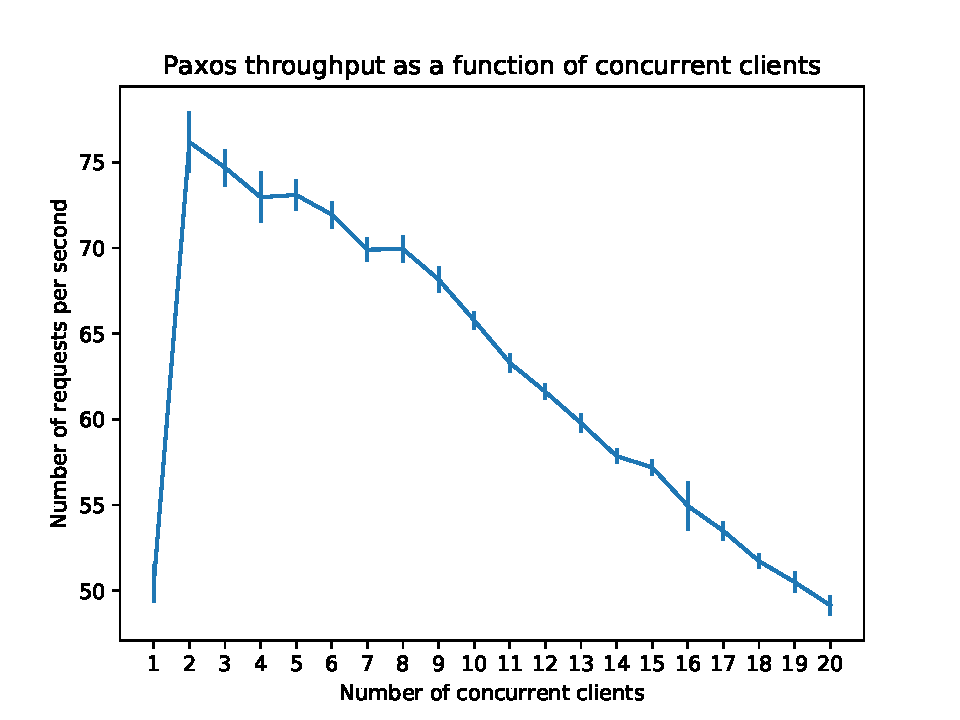
\includegraphics[width=0.48\textwidth]{figures/small_screen.pdf}
	\caption{Paxos throughput as a function of number of concurrent clients}
	\label{fig:paxos}
\end{figure}

\Fref{fig:paxos} shows the experimental results, where the vertical lines along the graph are errorbars given by the computed standard deviation.
As we can see, the throughput increase drastically from 1 to 2 clients due to them being concurrent.
When the number of concurrent clients increase further, the contention also increase which explains why the performance degrades.
While that is the case, the throughput with multiple concurrent clients is still higher than a single client until we reach 19 concurrent clients, which seem to yield approximately the same throughput.

\section{Conclusion}
% Concluding remarks
The Paxos consensus algorithm seem to scale well with concurrent clients, not degrading too quickly.
It scales very well from 1 to 2, and then degrades slowly as the number of concurrent clients increase.

\printbibliography
\end{document}
